\documentclass[Thesis.tex]{subfiles}
\begin{document}
\chapter{Parallelization}
\label{chp:parallelization}

Variational Monte Carlo calculations take a lot of computing power. It is easy
to set up a calculation that can take lifetimes to complete. Some systems are
simply to large for us to ever be able to work with, but at least we want to go
as far as possible. To do this we need to consider all available resources and
attempt to utilize them as efficiently as possible. This chapter is dedicated to
the various ways of speeding up calculations by means of parallelization.

Firstly we should make a few important notes. Parallelization is an effective
tool \emph{only} if we have more than one processing unit available. On a
single-core machine you may have the experience of multiple things
happening at once, but this is simply due to the single core switching back and
fourth faster than we can observe. This is \emph{concurrency}, or multitasking
as it is more often called when applied to humans. As we know, you are never
twice as productive when you attempt to do two things at once - often the
opposite is closer to the truth. The same is true for computers. So when we now
discuss ways of speeding up calculations by means of \emph{parallelization}, we are
at all times limited by the number of processing units available.

Lastly, we are going to make a distinction between two types of parallelization.
For any task that is not trivially parallel (i.e. two completely independent
tasks), we expect to need some sort of \emph{synchronization}, or communication
between the workers. We have two options for how to achieve this:

\begin{description}
\item[Shared memory:] Workers communicate through a shared section of memory, by
  reading/writing to it
  \item[Distributed memory:] Workers have independent memory sections, and
    communicate explicitly through sending/receiving messages (chunks of data)
\end{description}

\section{Distributed Memory}

The main bottle neck in VMC computations is the evaluation of expectation
values, such as \cref{eq:vmc-local-energy-formulation} and
\cref{eq:local-energy-gradient-alpha}. These calculations boil down to the
following basic algorithm:

\begin{enumerate}
\item Initialize sum $y = 0$
\item Sample new configuration, $\vX$\label{temp:1}
\item Add the output of some function, $y = y + f(\vX)$
\item Repeat from \ref{temp:1} for $n$ total steps
\item Let the result be $y_\text{final} = \flatfrac{y}{n}$
\end{enumerate}
The important note about this computation is that addition is commutative, and
so the order of the samples (obviously) does not matter. As such we could run
$p$ parallel processes, each of which computes $n / p$ terms before aggregating
the partials sums together and taking the mean.

This is a so called embarrassingly parallel problem, in the sense that it is
trivial to divide the workload up into smaller tasks. It has as close to linear
speedup potential\footnote{Linear speedup implies that if a task takes time $T$
to finish with one process, then it takes $T/n$ time with $n$ processes.} as one
can hope for, and is an ideal candidate for parallelization through distributed
memory multi processing. We want to run $p$ independent instances of the
algorithm, and pause momentarily to communicate the results. In the simple
example above, we just send the final partial sum acquired by each process. The
cost of sending the message is negligible compared to the main loop.

The main benefit of distributed memory is that it is easy to scale up to any
arbitrary number of machines, as long as they are connected in some way. These
machines could in principle be placed all around the world and still work well
for our purposes (some extra latency would be introduced by the distance).

\subsection{Implementation API: Message Passing Interface}

For the actual communication between distributed memory processes, we have the
standardized Message Passing Interface (MPI). This is typically implemented as a
set of C/C++ library functions with which we define the communication we want,
along with a special compiler (\texttt{mpicc/mpic++}) and a utility to start
multiple instances of a program (\texttt{mpiexec}\footnote{Quite common is the
  use of \texttt{mpirun}, however, this is not part of the MPI standard. The
  more stable and portable command is \texttt{mpiexec}.}).

\subsection{Example: Expectation Value of the Local Energy}

The following example is taken from the source code of QFLOW (\cref{chp:qflow}),
and illustrates a simply parallelized task: Computing the expected local energy.
While some details are specific to QFLOW's implementation, the general concept
should be clear.

\begin{lstfloat}
  \centering
\caption{Example excerpt from the source code of QFLOW, showing an MPI parallelized computation of the expected local energy.\citesource{qflow/hamiltonians/hamiltonian.cpp}}
\begin{lstlisting}[language=C++, label={lst:mpi-example}]
double Hamiltonian::local_energy(Sampler& sampler, Wavefunction& psi, long samples) const
{
    const int  n_procs = mpiutil::proc_count();
    const int  rank    = mpiutil::get_rank();
    const long samples_per_proc     // n / p + remainder.
      = samples/n_procs + (rank<samples % n_procs ? 1 : 0);

    double E_L = 0;

    for (long i = 0; i < samples_per_proc; ++i)
        E_L += local_energy(sampler.next_configuration(), psi);

    double global_E_L;
    MPI_Allreduce(
        &E_L, &global_E_L, 1, MPI_DOUBLE, MPI_SUM, MPI_COMM_WORLD);

    return global_E_L / samples;
}
\end{lstlisting}
\end{lstfloat}

To illustrate the speedup we obtain from using MPI parallelization, we have run
Listing~\ref{lst:mpi-example} on different number of cores. In particular, we computed
the local energy of a simple harmonic oscillator system of one particle in three
dimensions. \cref{fig:mpi-example} shows the number of MC iterations per second
as a function of the number of cores used. As advertised, we see a speedup that
follows closely the ideal linear curve.

Still, we should emphasize that in order to obtain these results, we had to
increase the total workload linearly with increasing number of CPUs. If we
don't, the task finishes so quickly that communication becomes a significant
part of the total time. So in order to fully utilize the power
of extra CPUs, we should make sure to structure the program such that the bulk of
it is spent in the independent parts of the program. In practice that means to
use a sufficiently large number of Monte Carlo samples.


\begin{figure}[h]
  \centering
    \resizebox{0.7\linewidth}{!}{%
        % This file was created by matplotlib2tikz v0.7.4.
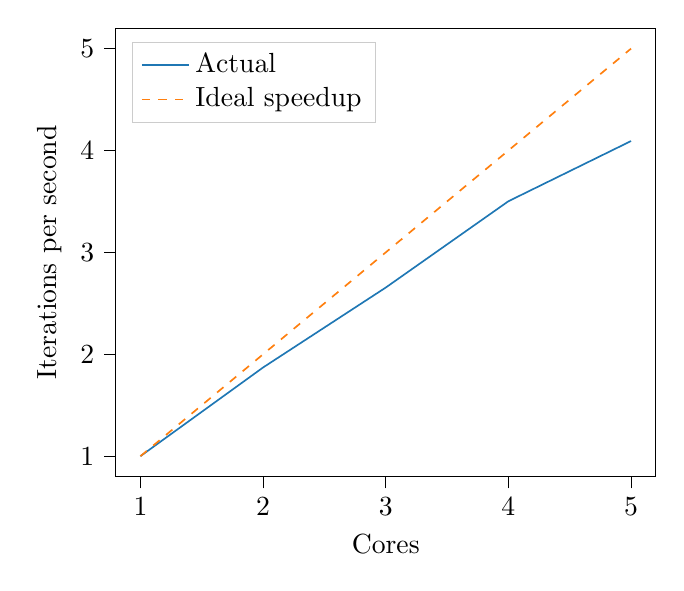
\begin{tikzpicture}

\definecolor{color0}{rgb}{0.12156862745098,0.466666666666667,0.705882352941177}
\definecolor{color1}{rgb}{1,0.498039215686275,0.0549019607843137}

\begin{axis}[
legend cell align={left},
legend style={at={(0.03,0.97)}, anchor=north west, draw=white!80.0!black},
tick align=outside,
tick pos=left,
x grid style={white!69.01960784313725!black},
xlabel={Cores},
xmin=0.8, xmax=5.2,
xtick style={color=black},
y grid style={white!69.01960784313725!black},
ylabel={Iterations per second},
ymin=0.8, ymax=5.2,
ytick style={color=black}
]
\addplot [semithick, color0]
table {%
1 1
2 1.87047656855767
3 2.65476945884948
4 3.50184341933712
5 4.09273731615231
};
\addlegendentry{Actual}
\addplot [semithick, color1, dashed]
table {%
1 1
2 2
3 3
4 4
5 5
};
\addlegendentry{Ideal speedup}
\end{axis}

\end{tikzpicture}
    }
  \caption[Speedup using MPI parallelization]{Iterations per second when running \cref{lst:mpi-example} with
varying number of processors. These results where obtained by running a test on
the Abel computing cluster. Exact results will vary greatly depending on the
availability of the cores, size of the workload and several other
factors.\citesource{writing/scripts/mpi-speed-test.py}}
  \label{fig:mpi-example}
\end{figure}


\section{Shared Memory}

As mentioned, the other possible way to allow for communication between workers
is through shared memory. This typically means running multiple threads within
the same process memory space, so that each thread has access to the same
memory. This is a faster type of communication compared with message passing,
but comes at the cost of having to consider data races. A data race occurs when
multiple workers try to access (with at least one write operation) the same
location in memory at the same time. The result of such behavior is undefined
and must be avoided.

\subsection{Implementation API: OpenMP}

Similarly to how distributed memory parallelization has the MPI standard, we
have the OpenMP standard for describing shared memory parallelization. The use
of this type of parallelization is typically made entirely through compiler
instructions embedded in the code, with some library functions also available.
The number of threads to use is decided at runtime, and can even change during
the course of the program. Importantly there is only one process running the
code, which lives for the duration of the program, and threads get
created and destroyed throughout the course of the computation.

\subsection{Example: Monte Carlo Estimation of $\pi$}
The following example shows a task equivalent in nature to
the one used in the last section, now parallelized using OpenMP.

\begin{lstfloat}
  \centering
  \caption{Example of parallel estimation of
$\pi$ using OpenMP. The example is complete and can be compiled as is.}
\begin{lstlisting}[language=C++, label={lst:openmp-example}]
#include <iostream>
#include <omp.h>
int main ()
{
    constexpr long steps = 1000000000;
    constexpr double step = 1.0 / (double) steps;

    int i, j;
    double x;
    double pi = 0;
#pragma omp parallel for reduction(+:pi) private(x)
    for (i=0; i < steps; i++)
    {
        x = (i+0.5)*step;
        pi += 4.0 / (1.0+x*x);
    }
    pi *= step;

    std::cout << "Pi = " << pi << std::endl;
}
\end{lstlisting}
\end{lstfloat}

Running Listing~\ref{lst:openmp-example} with a varying number of threads
results in \cref{fig:openmp-example} which shows how the speedup is about linear
until we run out of processing units (16 cores on the machine used), after which
it flattens out.

\begin{figure}[h]
  \centering
    \resizebox{0.7\linewidth}{!}{%
        % This file was created by matplotlib2tikz v0.7.4.
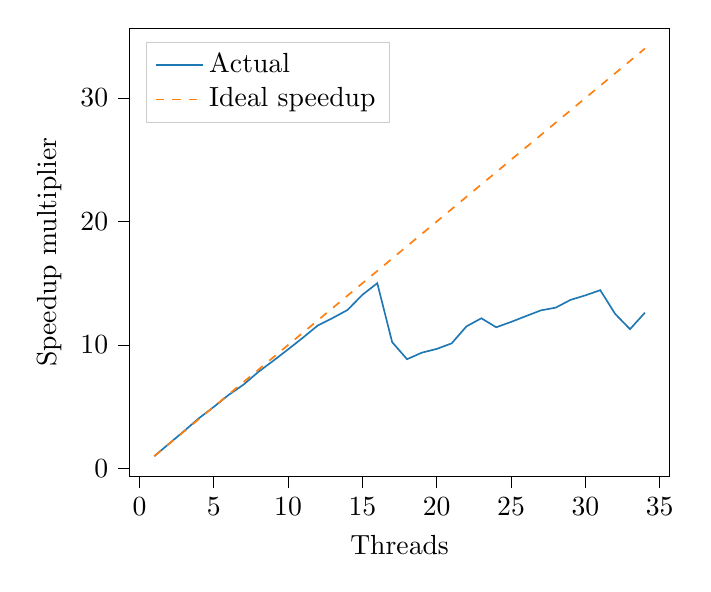
\begin{tikzpicture}

\definecolor{color0}{rgb}{0.12156862745098,0.466666666666667,0.705882352941177}
\definecolor{color1}{rgb}{1,0.498039215686275,0.0549019607843137}

\begin{axis}[
legend cell align={left},
legend style={at={(0.03,0.97)}, anchor=north west, draw=white!80.0!black},
tick align=outside,
tick pos=left,
x grid style={white!69.01960784313725!black},
xlabel={Threads},
xmin=-0.65, xmax=35.65,
xtick style={color=black},
y grid style={white!69.01960784313725!black},
ylabel={Speedup multiplier},
ymin=-0.65, ymax=35.65,
ytick style={color=black}
]
\addplot [semithick, color0]
table {%
1 1
2 2.01755412521943
3 3.02721685689201
4 4.06843657817109
5 4.98698293317906
6 5.95921189077083
7 6.78873794053948
8 7.82391649648287
9 8.7202832574608
10 9.64745383324007
11 10.5961893054702
12 11.5860215053763
13 12.1880523153058
14 12.8369322412509
15 14.0677274581803
16 15.0043516100957
17 10.2344909468685
18 8.85010266940452
19 9.38231292517007
20 9.68539325842697
21 10.1322362621217
22 11.5086782376502
23 12.166549047283
24 11.4361525704809
25 11.8691910499139
26 12.3407301360057
27 12.8035647976235
28 13.0260672459388
29 13.6554455445545
30 14.021960146401
31 14.4388609715243
32 12.5199709513435
33 11.282722513089
34 12.6161727039883
};
\addlegendentry{Actual}
\addplot [semithick, color1, dashed]
table {%
1 1
2 2
3 3
4 4
5 5
6 6
7 7
8 8
9 9
10 10
11 11
12 12
13 13
14 14
15 15
16 16
17 17
18 18
19 19
20 20
21 21
22 22
23 23
24 24
25 25
26 26
27 27
28 28
29 29
30 30
31 31
32 32
33 33
34 34
};
\addlegendentry{Ideal speedup}
\end{axis}

\end{tikzpicture}
    }
  \caption[Speedup using OpenMP parallelization]{Iterations per second when running \cref{lst:openmp-example} with
    varying number of processors. These results where obtained by running a test
    on the Abel computing cluster, on a node with 16 cores. We see a clear
    speedup until we run out of cores, at which point using more threads hurts
    performance.\citesource{writing/scripts/openmp_test.py}}
  \label{fig:openmp-example}
\end{figure}

This showcases how shared memory has excellent potential for speedup, but also
its major drawback: Scalability. It is considerably harder to scale a shared
memory architecture to an arbitrary number of processors because the ``shared''
part forces the processing units to be in relative close proximity to each
other.\footnote{You could in principle emulate shared memory for separate
  machines, but the emulation it self would have to use a message passing
  interface, which would defeat the purpose.} For this reason, we have focused
our parallelization efforts to MPI, because we anticipate the need for a large
number of parallel jobs. To some extent, a happy marriage of the two is
sometimes possible, but in general we expect that dedicating as many cores to
MPI processes as possible to be the most beneficial strategy.


\section{GPU Acceleration}

The final form of hardware acceleration we will mention is one that is
particularly central for ML in particular. While the two prior techniques boil
down to having multiple CPUs work together, certain tasks are particularly well
suited to acceleration by using a Graphics Processing Unit (GPU). These are
pieces of hardware typically designed to enable fast rendering of graphics for
computers, hence the name. They have a highly parallel structure optimized for
algorithms that need to process large blocks of data in parallel. A typical
example that relates to ML is matrix-matrix multiplication. Say we compute $\mat
C = \mat A \mat B$, or more explicitly:

\begin{align}
  C_{kl} = A_{ki}B_{il}.
\end{align}
The order in which we do any of the above $\mathcal{O}(n^3)$ operations really
doesn't matter, and so one can see how this can be an extremely parallel
process. A high-end GPU will have a number of cores in the four digit range,
facilitating speedups of several orders of magnitude compared to a CPU.

The recent (last decade) advancements in GPU technology has been an integral
part of the enormous amount of success in recent ML applications. Their use has
facilitated building models far beyond the capacity of an ordinary CPU.

\subsection{Implementation API: CUDA}

One popular way to program for a GPU is through CUDA, a programming
interface developed by NVIDIA. Similarly to MPI programming, its use is (for
C/C++) through a specialized compiler and some library functions. The typical
flow is to implement the parallel computation (say matrix-matrix multiplication
as above) in a dedicated CUDA function, and then call to this function from
regular code running on the CPU.

Many ML frameworks such as TensorFlow and PyTorch have built in support for GPU,
and offloading work to them is \say{trivial}. Unfortunately, we where unable to
use such frameworks in this work (mainly due to the reasons described in
\cref{chp:auto-diff}). Further, we have not actually implemented GPU support in
the current codes, despite this having large potential benefits. This is simply
a matter of time and realizing that it would require a considerable amount of effort
to get right. With the introduction of neural networks as wave functions, we see
no obvious reason why using GPUs would not cause significant speedups also in
our application of ML. The main challenge will likely be to join GPUs into the
existing MPI codes. We leave this a potential point of future work.



\end{document}
